\documentclass{beamer}
\usepackage[utf8]{inputenc}

\usepackage{utopia} %font utopia imported

\usetheme{Madrid}
\usecolortheme{default}


%------------------------------------------------
%Information to be included in the title page:
\title{Computer Architecture}

\subtitle{What computer contains and how it works}

\author{Nguyen The Minh}
\institute{Electronics and Computer Science Institute}
\date{Computing Conference, Oct 2050}

%\logo{
\includegraphics[height=1.5cm]{atom.png}}

%End of title page
%-------------------------------------------------

%------------------------------------------------------------
%The next block of commands puts the table of contents at the 
%beginning of each section and highlights the current section:

\AtBeginSection[]
{
  \begin{frame}
    \frametitle{Table of Contents}
    \tableofcontents[currentsection]
  \end{frame}
}
%------------------------------------------------------------

\begin{document}

\frame{\titlepage}

%---------------------------------------------------------
%This block of code is for the table of contents after
%the title page
\begin{frame}
\frametitle{Table of Contents}
\tableofcontents
\end{frame}
%---------------------------------------------------------

\section{Computer History}
\begin{frame}
\frametitle{Pre-20th Century}
\begin{columns}

\column{0.5\textwidth}
\begin{figure}[h!]
  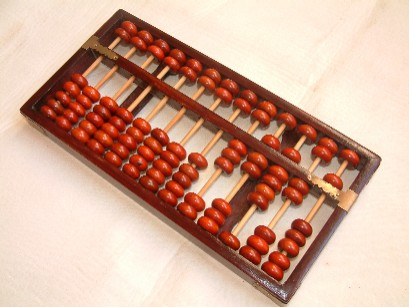
\includegraphics[height=2.5cm]{img/abacus.jpeg}
    \caption{A Chinese Abacus, 2nd BC}
\end{figure}
\column{0.5\textwidth}
\begin{figure}[h!]
  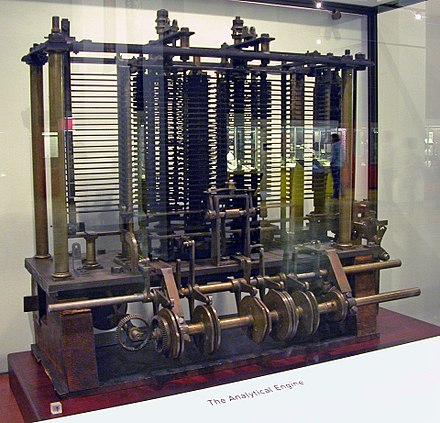
\includegraphics[height=2.5cm]{img/AnalyticalMachine.jpg}
    \caption{1833, Analytical Engine, London Museum}
\end{figure}
\end{columns}
\end{frame}

\section{Digital Computer}

\begin{frame}
\frametitle{First digital computer}
\begin{figure}[h!]
  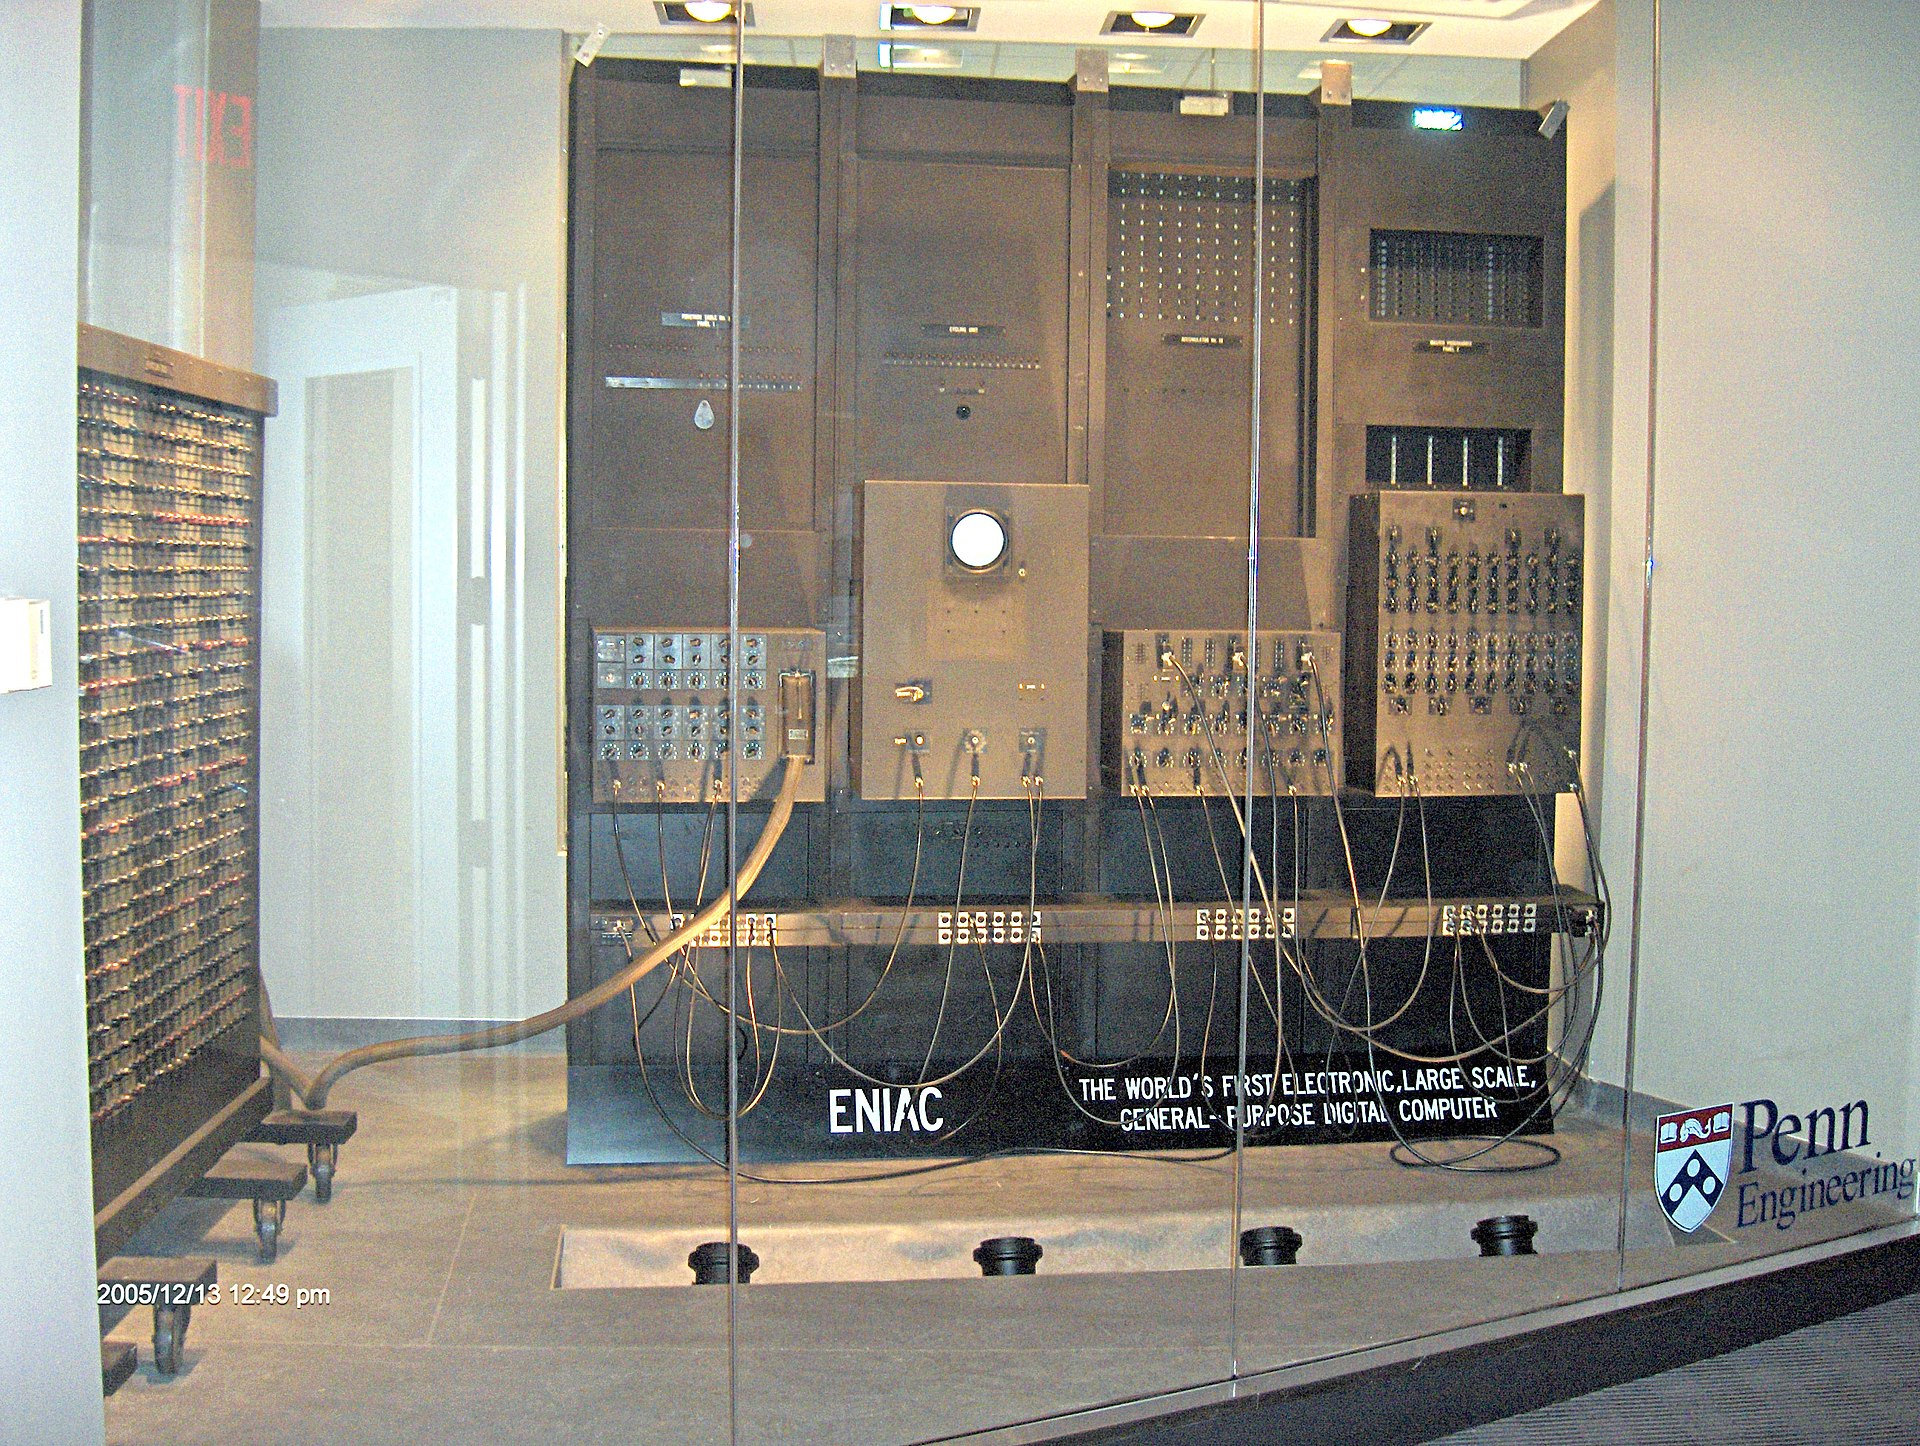
\includegraphics[height=2.5cm]{img/ENIAC.jpg}
    \caption{ENIAC - first electronic programmable computer - 1945}
\end{figure}
\end{frame}

\begin{frame}
\frametitle{Modern Digital Computer}
\begin{itemize}
    \item<1-> Text visible on slide 1
    \item<2-> Text visible on slide 2
    \item<3> Text visible on slides 3
    \item<4-> Text visible on slide 4
\end{itemize}
\end{frame}

%---------------------------------------------------------
%Example of the \pause command
\begin{frame}
In this slide \pause

the text will be partially visible \pause

And finally everything will be there
\end{frame}
%---------------------------------------------------------

\section{Instruction Set}

%---------------------------------------------------------
%Highlighting text
\begin{frame}
\frametitle{Sample frame title}

In this slide, some important text will be
\alert{highlighted} because it's important.
Please, don't abuse it.

\begin{block}{Remark}
Sample text
\end{block}

\begin{alertblock}{Important theorem}
Sample text in red box
\end{alertblock}

\begin{examples}
Sample text in green box. The title of the block is ``Examples".
\end{examples}
\end{frame}
%---------------------------------------------------------


%---------------------------------------------------------
%Two columns
\begin{frame}
\frametitle{Two-column slide}

\begin{columns}

\column{0.5\textwidth}
This is a text in first column.
$$E=mc^2$$
\begin{itemize}
\item First item
\item Second item
\end{itemize}

\column{0.5\textwidth}
This text will be in the second column
and on a second tought this is a nice looking
layout in some cases.
\end{columns}
\end{frame}
%---------------------------------------------------------


\end{document}